\lhead{\textbf{Basic Algorithms, Fall 2024 \\ CSCI-UA.0310-001}}
\chead{\Large{\textbf{Homework 4}}}
\def\lc{\left\lceil}   
\def\rc{\right\rceil}
\rhead{\textbf{Instructor: Rotem Oshman \\ Name: Ishan Pranav}}
\runningheadrule
\firstpageheadrule
\cfoot{}

\newcommand{\True}{\mathtt{true}}
\newcommand{\False}{\mathtt{false}}

\subsection*{References}

Collaborated with Crystal Huang.

\subsection*{Question 1: $k$-th Smallest Element from Two Lists}

Suppose you are given two \emph{sorted} lists $A[1,\ldots,n]$ and $B[1,\ldots,m]$ of size $n$ and $m$, respectively. Give an $O(\log k)$ algorithm to find the $k$-th
smallest element in $A \cup B$, i.e., of the combination of the two arrays. For simplicity, you can assume $k \leq \min(m,n)$. Justify the correctness and running time of your algorithm. 

\begin{solution}\\

\noindent\textbf{Algorithm. }{\sc FindIndex}($A,B,k$) where $A[1,\dots,n],B[1,\dots,m]$ are sorted lists and $k\in\mathbb{N}$ where $k\leq\min(n,m)$. That is, for all $1\leq i<n$, we have $A[i]\leq A[i+1]$, and for all $1\leq j<m$, we have $B[j]\leq B[j+1]$:
\begin{itemize}
\item if $n=0$, then return $B[k]$;
\item if $m=0$, then return $A[k]$;
\item if $k=1$, then return $\min(A[1],B[1])$;
\item otherwise, for $k>1$, compute $i\leftarrow\left\lfloor\frac{k}{2}\right\rfloor$. Then:
\begin{itemize}
\item if $A[i]\leq B[i]$, then return {\sc FindIndex}($A[i+1,\dots,n],B[1,\dots,m],k-i$);
\item otherwise, return {\sc FindIndex}($A[1,\dots,n],B[i+1,\dots,m],k-i$).
\end{itemize}
\end{itemize}

\noindent\textbf{Proposition I.}

\noindent\textit{Claim. }For all sorted lists $A[1,\dots,n],B[1,\dots,m]$ and all $k\leq\min(n,m)$, {\sc FindIndex}($A,B,k$) returns $C[k]$, where $C=~${\sc Merge}($A,B$), the result of the well-known {\sc Merge} algorithm. That is, {\sc FindIndex}($A,B,k$) returns the $k$-th element of the sorted list that contains all elements of sorted lists $A$ and $B$ (and no other elements). Note $k\geq 1,m\geq 0,n\geq 0$.\\

\noindent\textit{Proof.}
\begin{itemize}
\item Suppose $n=0$. Then $m\geq 1$. Consider $C[1,\dots,m]$, the result of merging $A$ and $B$. Since $n=0$, we know $C=B$. For all $k\in\mathbb{N}$, {\sc FindIndex}($A,B,k$) returns $B[k]=C[k]$. Thus, when $n=0$, the claim holds for all $k\in\mathbb{N}$.
\item Suppose $m=0$. Then $n\geq 1$. Consider $C[1,\dots,n]$, the result of merging $A$ and $B$. Since $m=0$, we know $C=A$. For all $k\in\mathbb{N}$, {\sc FindIndex}($A,B,k$) returns $A[k]=C[k]$. Thus, when $m=0$, the claim holds for all $k\in\mathbb{N}$.
\item Suppose instead $m>0$ and $n>0$. We can demonstrate the claim for $m>0$ and $n>0$ by induction on $k$.\\

\textit{Basis. }Consider $k=1$. Consider also $C[1,\dots,m+n]$, the result of merging $A$ and $B$. The least element in $C$ is either the least element in $A$ or the least element in $B$; specifically, it is the smaller of the least element in $A$ and the least element in $B$. Of course, in this case {\sc FindIndex}($A,B,k$) returns $\min(A[1],B[1])$. Since $A,B$ are sorted lists, $A[1]$ is the least element in $A$ and $B[1]$ is the least element in $B$. Therefore {\sc FindIndex}($A,B,k$) returns the first smallest element in $C$. Since $k=1$, the basis holds for all $A[1,\dots,n],B[1,\dots,m]$.\\

\textit{Hypothesis. }Consider $1<k\leq\ell<\min(n,m)$. Assume that for all sorted lists $A[1,\dots,n]$ and $B[1,\dots,n]$, {\sc FindIndex}($A,B,\ell$) returns the $\ell$-th element of the sorted list that contains all elements of $A$ and $B$ (and no other elements).\\

\textit{Inductive step. }Consider $k=\ell+1$. For all sorted lists $A[1,\dots,n],B[1,\dots,m]$, we have $i=\left\lfloor\frac{\ell+1}{2}\right\rfloor$. Consider $C[1,\dots,m+n]$, the result of merging $A$ and $B$.
\begin{itemize}
\item Suppose $A[i]\leq B[i]$. Since $A$ and $B$ are sorted, and since $A[i]\leq B[i]$, we know that the $(\ell+1)$-th element in $C$ is definitely not within the first $i$ elements of $A$. We can ignore the first $i$ elements in $A$, adjusting our index in the subarray from $\ell+1$ to $\ell+1-i$ (to account for the $i$ elements excluded, which precede it in sorted order).

The result for the new subarray is given by {\sc FindIndex}($A[i+1,\dots,n],B[1,\dots,m],k-i$), which is the return value of the algorithm in this case. By the strong induction hypothesis, the claim holds for this result.
\item Suppose instead $A[i]>B[i]$. Since $A$ and $B$ are sorted, and since $B[i]<A[i]$, we know that the $(\ell+1)$-th element in $C$ is definitely not within the first $i$ elements of $B$. We can ignore the first $i$ elements in $B$, adjusting our index in the subarray from $\ell+1$ to $\ell+1-i$ (to account for the $i$ elements excldued, which precede it in sorted order).

The result for the new subarray is given by {\sc FindIndex}($A[1,\dots,n],B[i+1,\dots,m],k-i$), which is the return value of the algorithm in this case. By the strong induction hypothesis, the claim holds for this result.
\end{itemize}

In all cases, {\sc FindIndex}($A,B,\ell+1$) returns the ($\ell+1$)-th element of the sorted list that contains all elements of $A$ and $B$ (and no other elements), thus completing the inductive step.

Hence, by the principle of mathematical induction, the claim holds for all $k\in\mathbb{N}$ when $m>0$ and $n>0$.
\end{itemize}

\noindent We have shown that for all sorted lists $A[1,\dots,n],B[1\dots,m],n\geq 0,m\geq 0,k\in\mathbb{N}$, if $k\leq\min(n,m)$, then {\sc FindIndex}($A,B,k$) returns the $k$-th element of the sorted list that contains all elements of sorted lists $A$ and $B$.$~\square$\\

\noindent\textbf{Proposition II.}

\noindent\textit{Claim. }For all sorted lists $A[1,\dots,n],B[1,\dots,m]$ and all $k\leq\min(n,m)$, the running time of {\sc FindIndex}($A,B,k$) is $T(k)=O(\log{k})$.\\

\noindent\textit{Proof. }On each recursive level, {\sc FindIndex}($A,B,k$) performs a constant number of operations: At most, one element from $A$ is compared with one element from $B$. So the work done on each level is $\Theta(1)$. Since $k$ is reduced by roughly half on each recursive call, the number of levels is asymptotically $\log_2k$. From this intuition, we can guess that the running time of {\sc FindIndex}($k$), $T(k)$ may be $O(\log_2k)$. 

We can use a recurrence to estimate $T(k)$:
\begin{align*}
T(1)&=\Theta(1),&
T(k)&=T\left(\left\lfloor\frac{k}{2}\right\rfloor\right)+\Theta(1),
\text{ for }k>1.
\end{align*}
We want to show that $T(k)=O(\log_2k)$. That is, we want to show that there exist positive constants $C,n_0$ such that $T(k)\leq C\log{k}$ for all $k\geq n_0$. Taking $k_0=2$, we can demonstrate this claim for all $k>2$ by induction on $k$.\\

\noindent\textit{Basis. }Consider $k=2$. Observe
\begin{align*}
T(2)&=T\left(\left\lfloor\frac{2}{2}\right\rfloor\right)+\Theta(1)\\
&=T(1)+\Theta(1)\\
&=\Theta(1)+\Theta(1)&\textit{asymptotically,}\\
&=c_1+c_2&\textit{where $c_1,c_2$ are positive constants.}
\end{align*}

\noindent Since $T(2)=c_1+c_2$, we can choose any $C\geq\frac{c_1+c_2}{\log_2{k}}$ so that $T(2)\leq C\log_2{k}$. The claim holds in the base case.\\

\noindent\textit{Hypothesis. }Consider $2<\ell\leq k$. Assume that $T(\ell)=O(\log_2\ell)$.\\

\noindent\textit{Inductive step. }Consider $k=\ell+1$. Observe
\begin{align*}
T(\ell+1)
&=T\left(\left\lfloor\frac{\ell+1}{2}\right\rfloor\right)+\Theta(1)\\
&=O\left(\log_2\left\lfloor\frac{\ell+1}{2}\right\rfloor\right)+\Theta(1)&\textit{from the strong inductive hypothesis,}\\
&\leq C\log_2\left(\left\lfloor\frac{\ell+1}{2}\right\rfloor\right)+\Theta(1)\\
&\leq C\log_2\left(\left\lfloor\frac{\ell+1}{2}\right\rfloor\right)+\Theta(1)\\
&\leq C\log_2\ell+\Theta(1)&\textit{for $C>0$ and $\ell\geq 2,$}\\
&=O(\log_2\ell)+\Theta(1)\\
&=O(\log_2\ell)&\textit{asymptotically.}
\end{align*}

\noindent This completes the inductive step.\\

\noindent Hence, by the principle of mathematical induction, we have $k_0=2,C\geq\frac{c_1+c_2}{\log_2k}$ for which $T(k)\leq C\log_2k$ for all $k\geq k_0$.\\

\noindent Therefore, $T(k)=O(\log_2k)=O(\log k)$.$~\square$
\end{solution}
\subsection*{Question 2: Permutations}

Define the notation $[n] = \{1, 2, \ldots, n\}$, and let $S_n$ be the set of all possible permutations of $[n]$. The size of $S_n$ is given by $|S_n|=n!=n\cdot (n-1) \cdots 1$. Recall that $n!=O(n^n)$ and $2^n=O(n!)$. 
Now, each input in $S_n$ can serve as an input for a sorting algorithm. Instead of a perfectly correct sorting algorithm, we will look at a class of algorithms that only produce a sorted result on some of the inputs. More concretely, we say that a sorting algorithm is $\eps$-correct if the algorithm produces the correct result (i.e., produces a sorted array as output) on exactly $\eps$ fraction of the set of inputs in $S_n$. In other words, an $\eps$-correct sorting algorithm is one that produces the correct result on $\eps \cdot (n!)$ possible inputs and produces an incorrect result otherwise.
\begin{enumerate}
    \item Show that for any $0\leq \epsilon\leq 1$, the decision tree of an $\epsilon$-correct comparison-based sorting algorithm must have at least $\epsilon \cdot n!$ leaves.
\begin{solution}
\textit{Claim. }Let $0\leq\epsilon\leq 1$. Then the decision tree of an $\epsilon$-correct comparison-based sorting algorithm must have at least $\epsilon\cdot n!$ leaves.

\textit{Proof. }Assume, for the sake of contradiction, that there exists some $\epsilon$-correct sorting algorithm {\sc HypotheticalSort} for which the number of leaves is less than $\epsilon\cdot n!$. Since {\sc HypotheticalSort} is an $\epsilon$-correct sorting algorithm, it produces correct solutions for $\epsilon\cdot n!$ possible inputs. Every input array $A$ has exactly one correct sorted solution $A_{\rm sorted}$. Since {\sc HypotheticalSort} produces correct results for $\epsilon\cdot n!$ possible inputs, it produces exactly $1\cdot\epsilon\cdot n!=\epsilon\cdot n!$ possible outputs. In a recursive decision tree, each leaf corresponds to a single output. Therefore, the decision tree of {\sc HypotheticalSort} has $\epsilon\cdot n!$ leaves. This contradicts the hypothesis that {\sc HypotheticalSort} has less than $\epsilon\cdot n!$ leaves.

Therefore for all $0\leq\epsilon\leq 1$, the decision tree of an $\epsilon$-correct comparison-based sorting algorithm must have at least $\epsilon\cdot n!$ leaves.$~\square$
\end{solution}
\end{enumerate}
\newpage

\noindent
In the following, we want to investigate whether lowering $\eps$ can yield a saving in the number of comparisons required by a sorting algorithm. Intuitively if the algorithm only has to be correct on a certain fraction of inputs this should speed up the algorithm. For instance, an algorithm that does not need to be correct at all clearly does not need $\Omega(n \log n)$ comparisons. \hint{Use the number of leaves in the decision tree to derive a lower bound on its height.} 

\begin{enumerate}[resume]
    \item Let $\eps=1/2$. Show that for any constant $C\geq 0$, there is no comparison-based $\eps$-correct sorting algorithm that can sort using less than $C \cdot n$ comparisons. This shows that taking $\eps=1/2$ does not help us reduce the number of comparisons to linear. 
\begin{solution}
\textit{Claim. }Let $\epsilon=\frac{1}{2}$. Then for any $C\geq 0$, there is no comparison-based $\epsilon$-correct sorting algorithm that can sort using less than $Cn$ comparisons.

\textit{Proof. }Assume, for the sake of contradiction, that there exists some comparison-based $\epsilon$-correct sorting algorithm {\sc HypotheticalSort} that can sort using less than $Cn$ comparisons for $\epsilon=\frac{1}{2}$. Then the number of leaves in its decision tree is at least $\epsilon\cdot n!=\frac{1}{2}\cdot n!=\frac{n!}{2}$. Thus, the height of this tree $H(n)$ is at least on the order of $\log{\frac{n!}{2}}$. Note
\begin{align*}
\frac{n!}{2}\geq\frac{\left(\frac{n}{2}\right)^{\frac{n}{2}}}{2}.\\
\end{align*}
Observe
\begin{align*}
H(n)&\geq\log\frac{n!}{2}\\
&\geq\log\frac{\left(\frac{n}{2}\right)^{\frac{n}{2}}}{2}\\
&\geq\log\left(\frac{n}{2}\right)^{\frac{n}{2}}-\log 2\\
&\geq\frac{n}{2}\log\frac{n}{2}-\log 2.
\end{align*}

We have $C_1\left(\frac{n}{2}\log\frac{n}{2}-\log 2\right)\geq n\log n$ for all $n\geq n_0$, taking $C_1>3$ and large enough $n_0$.

Thus, $H(n)=\Omega(n\log n)=\Omega(n)$. Therefore {\sc HypotheticalSort} sorts using greater than or equal to $Cn$ comparisons for some $C=C_1$. This contradicts the hypothesis that {\sc HypotheticalSort} can sort using less than $Cn$ comparisons for all $C\geq 0$.

Therefore, when $\epsilon=\frac{1}{2}$, for all $C\geq 0$, there is no comparison-based $\epsilon$-correct sorting algorithm that can sort using less than $Cn$ comparisons.$~\square$
\end{solution}
\newpage
    \item Consider $\eps=1/n$. In this setting, are we able to achieve a sorting algorithm for $S_n$ with $O(n)$ comparisons? Justify your answer.
\begin{solution}
\textit{Claim. }Let $\epsilon=\frac{1}{n}$. Then for any $C\geq 0$, there is no comparison-based $\epsilon$-correct sorting algorithm that can sort using $O(n)$ comparisons---that is, less than or equal to $Cn$ comparisons.

\textit{Proof. }Assume, for the sake of contradiction, that there exists some comparison-based $\epsilon$-correct sorting algorithm {\sc HypotheticalSort} that can sort using less than or equal to $Cn$ comparisons for $\epsilon=\frac{1}{n}$. Then the number of leaves in its decision tree is at least $\epsilon\cdot n!=\frac{1}{n}\cdot n!=(n-1)!$. Thus, the height of this tree $H(n)$ is at least on the order of $\log((n-1)!)$. Note
\begin{align*}
(n-1)!\geq\left(\frac{n-1}{2}\right)^{\frac{n-1}{2}}.\\
\end{align*}
Observe
\begin{align*}
H(n)&\geq\log((n-1)!)\\
&\geq\log\left(\frac{n-1}{2}\right)^{\frac{n-1}{2}}\\
&\geq\frac{n-1}{2}\log\frac{n-1}{2}.
\end{align*}

We have $C_1\left(\frac{n-1}{2}\log\frac{n-1}{2}\right)>n\log n$ for all $n\geq n_0$, taking $C_1\geq 3$ and large enough $n_0$.

Thus, $H(n)=\omega(n\log n)$. We know that $\omega(n\log n)=\omega(n)$ is strictly greater than $O(n)$ for large enough $n$. Therefore {\sc HypotheticalSort} sorts using greater than $Cn$ comparisons for some $C=C_1$. This contradicts the hypothesis that {\sc HypotheticalSort} can sort using $O(n)$ comparisons.

Therefore, when $\epsilon=\frac{1}{n}$, for all $C\geq 0$, there is no comparison-based $\epsilon$-correct sorting algorithm that can sort using $O(n)$ comparisons.$~\square$
\end{solution}
\newpage
    \item Consider $\eps=\frac{1}{2^n}$. In this setting, are we able to achieve a sorting algorithm for $S_n$ with $O(n)$ comparisons? Justify your answer.
\begin{solution}
\textit{Claim. }Let $\epsilon=\frac{1}{2^n}$. Then for any $C\geq 0$, there is no comparison-based $\epsilon$-correct sorting algorithm that can sort using $O(n)$ comparisons---that is, less than or equal to $Cn$ comparisons.

\textit{Proof. }Assume, for the sake of contradiction, that there exists some comparison-based $\epsilon$-correct sorting algorithm {\sc HypotheticalSort} that can sort using less than or equal to $Cn$ comparisons for $\epsilon=\frac{1}{2^n}$. Then the number of leaves in its decision tree is at least $\epsilon\cdot n!=\frac{1}{2^n}\cdot n!=\frac{n!}{2^n}$. Thus, the height of this tree $H(n)$ is at least on the order of $\log\left(\frac{n!}{2^n}\right)$. Note
\begin{align*}
\frac{n!}{2^n}\geq\frac{\left(\frac{n}{2}\right)^{\frac{n}{2}}}{2^n}.\\
\end{align*}
Observe
\begin{align*}
H(n)&\geq\log\left(\frac{n!}{2^n}\right)\\
&\geq\log\frac{\left(\frac{n}{2}\right)^{\frac{n}{2}}}{2^n}\\
&\geq\log\left(\frac{n}{2}\right)^{\frac{n}{2}}-\log2^n\\
&=\frac{n}{2}\log\frac{n}{2}-n\log 2.
\end{align*}

We have $C_1\left(\frac{n}{2}\log\frac{n}{2}-n\log 2\right)>n\log n$ for all $n\geq n_0$, taking $C_1\geq 10$ and large enough $n_0$.

Thus, $H(n)=\omega(n\log n)$. We know that $\omega(n\log n)=\omega(n)$ is strictly greater than $O(n)$ for large enough $n$. Therefore {\sc HypotheticalSort} sorts using greater than $Cn$ comparisons for some $C=C_1$. This contradicts the hypothesis that {\sc HypotheticalSort} can sort using $O(n)$ comparisons.

Therefore, when $\epsilon=\frac{1}{2^n}$, for all $C\geq 0$, there is no comparison-based $\epsilon$-correct sorting algorithm that can sort using $O(n)$ comparisons.$~\square$
\end{solution}
\newpage 
    \item Consider $\eps=\frac{2^n}{n!}$. In this setting, are we able to achieve a sorting algorithm for $S_n$ with $O(n)$ comparisons?
\begin{solution}
\textit{Claim. }Let $\epsilon=\frac{2^n}{n!}$. Then for any $C\geq 0$, there exists a comparison-based $\epsilon$-correct sorting algorithm that can sort using $O(n)$ comparisons---that is, less than or equal to $Cn$ comparisons.

\textit{Proof. }Let {\sc Sort} be a comparison-based $\epsilon$-correct sorting algorithm that can sort using less than or equal to $Cn$ comparisons for $\epsilon=\frac{2^n}{n!}$. Then the number of leaves in its decision tree is at least $\epsilon\cdot n!=\frac{2^n}{n!}\cdot n!=2^n$. Thus, the height of this tree $H(n)$ is at least on the order of $\log 2^n=n\log 2$. Observe
\begin{align*}
H(n)&\geq n\log 2.
\end{align*}
We have $n\log{2}\leq Cn$ for $C\geq\log{2}$ for all $n\geq 0$. Thus, $H(n)=O(n)$, so {\sc Sort} can sort using $O(n)$ comparisons.$~\square$
\end{solution}
\end{enumerate}
\newpage
\subsection*{Question 3: Disjointed arrays}
Let $A[1,\ldots,m]$ and $B[1,\ldots,n]$ be two sorted
arrays each containing distinct elements. Let
$m\leq n$ and $n$ is a multiple of $m$. 
The problem is to determine if the two arrays
are disjointed or not. Two arrays are said
to be disjointed if their intersection is
$\emptyset$. 

\begin{enumerate}
	\item Let us assume that $A$ and $B$ are disjoint.
	We define $C$ as the sorted combination of
	$A$ and $B$, i.e., $C=A\cup B$ and $C$ is sorted. Clearly,
	$|C|=m+n$ because $A\cap B=\emptyset$. Define
	$D$ of length $m+n$ where $D[i]=1$ if $C[i]\in A$ and 0
	otherwise. Give a count of the number of such possible
	arrays $D$. Justify your answer. 

\begin{solution}
\textbf{Proposition 3.1.}
\textit{Claim. }Let $A[1,\dots,n],B[1,\dots,m]$ be sorted arrays containing distinct elements where $m\leq n$ and $n$ is a multiple of $m$. Let $C=A\cup B$ where $C$ is sorted and $D[1,\dots,m+n]$ where $D[i]=1$ if $C[i]\in A$, and $C[i]=0$ otherwise, for $1\leq i\leq m+n$.

\textit{Proof. }Since $C=A\cup B$, we know $D[i]=1$ if $C[i]\in A$ or $0$ if $C[i]\in B$. There are $m+n$ many elements in $D$, and for each element, it is either in $A$ or not in $A$. It is known that there are $n$ elements in $A$, so $n$ of $m+n$ elements must be chosen to be $1$ and the remaining $m$ elements must be $0$.

Thus, the number of such possible arrays is $\binom{m+n}{n}=\binom{m+n}{m}$.$~\square$
\end{solution}
\newpage
\item We go back to the original problem---we do not know whether $A,B$ are disjoint. Let us assume that $A$ contains 1 element, and $B$ contains 2 elements. 

\begin{itemize}
\item Draw a comparison-based decision tree for this problem.
\item You will also present a modification of the above tree
where you will change the label of every leaf node marked as $\True$ 
with a corresponding array $D$. 
\end{itemize}

You will ensure that your decision tree makes 
the least number of comparisons possible and has
the shortest height possible. The internal 
node will be of the form $(i,j)$ which 
indicates that you are comparing $A[i]$ and $B[j]$. 
Now, each such internal node will have three children---one corresponding to $A[i]<B[j]$, one corresponding to $A[i]=B[j]$,
and one corresponding to $A[i]>B[j]$. The leaf
nodes will contain the values $\True,\False$
where $\True$ indicates that $A,B$ are disjoint
and $\False$ indicates the opposite.
\begin{figure}[h]
\centering
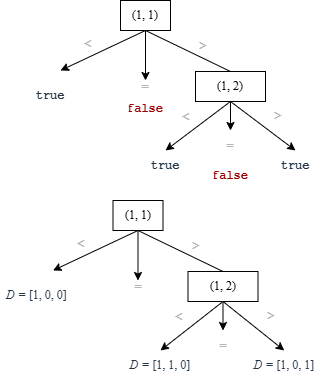
\includegraphics[width=9.5cm]{../images/hw4-3-2.png}
\caption{\textit{Top: }A comparison-based decision tree for this problem. \textit{Bottom: }A modification of the above tree where the label of every leaf node marked as $\True$ is replaced with a corresponding array $D$.}
\label{fig:hw4_3_20}
\end{figure}
\begin{solution}
Please see Figure~\ref{fig:hw4_3_2}.
\end{solution}
\newpage

\item Now we look at the general problem, i.e.,
for any $m,n$. It can be shown that the decision
tree for this general problem will have every
leaf node labeled $\True$ correspond with
a distinct array $D$, as defined in part (1).
This is in fact a bijective mapping, i.e., every
leaf node labeled $\True$ has a corresponding array $D$
and every array $D$ has a corresponding leaf node
labeled $\True$
Now, using this and your answer from part (1),
show that problem has a worst-case lower
bound of $\Omega(m\log(1+n/m))$.
\begin{solution}\textbf{Proposition 3.3. }\textit{Definitions. }Let $A[1,\dots,n],B[1,\dots,m]$ be sorted arrays containing distinct elements where $m\leq n$ and $n$ is a multiple of $m$. Let $C=A\cup B$ where $C$ is sorted. Let $D[1,\dots,m+n]$ be an array where $D[i]=1$ if $C[i]\in A$ and $0$ otherwise.

\textit{Axiom I. }There exists a bijective mapping between nodes labeled $\True$ and possible arrangements of $D$. For each node labeled $\True$, there is exactly one arrangement of $D$. For each arrangement of $D$, there is exactly one node labeled $\True$.

\textit{Axiom II. }$\binom{a}{b}\geq\left(\frac{a}{b}\right)^b$ for $a\geq b\geq 1$. This follows from $b^b\geq b!$ for all $b\geq 1$.

\textit{Claim. }The problem has a worst-case lower bound of $\Omega\left(m\log\left(1+\frac{n}{m}\right)\right)$.

\textit{Proof. }Let $H(n,m)$ denote the height of the decision tree in the worst case. Since each internal node has three children---one corresponding to $A[i]<B[j]$, one coprresponding to $A[i]=B[j]$, and one corresponding to $A[i]>B[j]$---this is a ternary tree with height equal to the ternary logarithm of the number of leaves.

From Proposition 3.1, we know there are $\binom{m+n}{m}$ arrangements of $D$. From Axiom I, there are as many arrangements of $D$ as nodes labeled $\True$. Therefore there are $\binom{m+n}{m}$ nodes labeled $\True$.

The worst case occurs when $A$ and $B$ are disjoint. Suppose not: Then $A[i]=B[j]$ for some $i,j$, and the result is $\False$. We can choose different inputs $A,B'$, where $B'[1,\dots,m]=[B[1],\dots,B[j-1],x,B[j+1],\dots B[m]]$ and $x\neq A[i]$. In other words, we can replace $B'[j]$ with some $x$ to make $A$ and $B'$ disjoint and perform the algorithm again on $A$ and $B'$. Now $A[i]\neq B[j]$, so at least one additional comparison is performed. The running time will be as bad, or worse, than when $A$ and $B$ are not disjoint. So the worst case is when $A$ and $B$ are disjoint.

When $A$ and $B$ are disjoint, the result is $\True$. There are $\binom{m+n}{m}$ nodes labeled $\True$, so in the worst case all $\log_3\binom{m+n}{n}$ levels must be visited before the last evaluation concludes that $A$ and $B$ are disjoint. Intuitively, this corresponds to the case where the first $m-1$ elements compared between $A$ and $B$ are different, but the last element compared is identical.

Observe:

\begin{align*}
H(n,m)&\geq\log_3\binom{m+n}{m}\\
&\geq\log_3\left(\frac{m+n}{m}\right)^m&\textit{from Axiom II, since $n\geq m\geq 1$,}\\
&\geq\log_3\left(1+\frac{n}{m}\right)^m\\
&\geq m\log_3\left(1+\frac{n}{m}\right)\\
&\geq\frac{1}{\log{3}}\cdot m\log\left(1+\frac{n}{m}\right).
\end{align*}

There exists a constant $\frac{1}{\log{3}}>0$ for which $H(n,m)\geq\frac{1}{\log{3}}\cdot m\log\left(1+\frac{n}{m}\right)$ for large enough $m$ (and, since $n\geq m$, large enough $n$).

Therefore, $H(n,m)=\Omega(m\log(1+n/m))$. Of course, the work done on each level is constant.

Ergo the problem has a worst-case lower bound of $\Omega(m\log(1+n/m)).~\square$
\end{solution}
\end{enumerate}